
\documentclass[12pt,italian,a4paper,oneside,openright]{book}
\usepackage{url,amsfonts,epsfig}
\usepackage[italian]{babel}
\usepackage[utf8]{inputenc}
\usepackage{vmargin}
\usepackage{amsmath}
\usepackage{indentfirst}
\usepackage{graphicx}
\graphicspath{{img/}}
\usepackage[hyperindex]{hyperref} %per l'indice interattivo
\hypersetup{colorlinks=true, linkcolor=black} %per colorare i link
\DeclareGraphicsRule{.jpg}{jpg}{}{} %da commentare per il PDF
\setmarginsrb{35mm}{30mm}{30mm}{30mm}{0mm}{10mm}{0mm}{10mm}
%%\setmarginsrb{1.5cm}{1.5cm}{1,2cm}{1,5cm}{0cm}{2cm}{2cm}{2cm}


\title{Template per la tesina in .tex}
\author{Nome e Cognome}
\date{Data di esame}

\begin{document}
\pagenumbering{Roman}

\baselineskip 1.5em

{ \thispagestyle{empty}


\vskip 1cm \large \centerline{\textsc{Università degli Studi di Napoli ``Parthenope''}}

\centerline {\textsc{Facoltà di Scienze e Tecnologie}}

\centerline {\small\textsc{Corso di laurea in Informatica}}

\begin{center}

\includegraphics[scale=0.24]{logo_parthenope.png}
\end{center}

\vskip 0.5cm

\large \centerline {\textsc{Progetto di Reti di Calcolatori}}

\vskip 0.5cm

\Large \centerline {PropertEase}


\vskip 4.5cm


\large
\begin{minipage}[t]{7cm}
\textsc{Docente}

Emanuel Di Nardo\\

\end{minipage}
\hfill
\begin{minipage}[t]{8cm}
    \textsc{Studenti e matricole}

    Amore Gabriel - 0124002585 \\
    Ben Baccar Alexandr - 0124002586 \\
    De Micco Carmine - 0124002630 \\
\end{minipage}

\vskip 2.0 cm \Large \centerline {Anno Accademico 2023-2024}
\vfill \eject}

\markboth{Indice}{Indice}
\tableofcontents
%%\listoffigures
%%\listoftables
\newpage

\pagenumbering{arabic}
\thispagestyle{headings}

\chapter{Traccia progetto} \label{trac}
\noindent Si vuole sviluppare un sistema software per per un'agenzia immobiliare che offre servizi di vendita di proprietà e consulenze da parte di professionisti.
\\
Ogni immobile ha caratteristiche come \textbf{indirizzo, metratura, descrizione, ascensori, numero di vani, accessori, giardini e terrazzi.}
\\\\
Le case sono suddivise in:
\begin{itemize}
\item \textbf{Appartamento:} inteso come un locale in un condominio;
\item \textbf{Casa indipendente:} inteso come una villetta;
\item \textbf{Garage:} inteso come spazio non adibito al domicilio.
\end{itemize}
Il sistema deve essere gestito in modalità \textbf{amministratore} e in modalità \textbf{cliente} (e.g. operazioni sul web).
\\\\
L'\textbf{amministratore}, inteso come un \textit{agente immobiliare}, può effettuare le seguenti operazioni:
\begin{itemize}
    \item Visualizzare, inserire, modificare ed eliminare un immobile con le relative informazioni;
    \item Inserire le date in cui è disponibile per appuntamenti con i clienti;
    \item Visualizzare ed eliminare gli appuntamenti presi con i clienti.
\end{itemize}
Il \textbf{cliente} può effettuare le seguenti operazioni:
\begin{itemize}
    \item Visualizzare gli immobili;
    \item Prendere appuntamenti con gli amministratori nel limite di quelle messe a disposizione da questi ultimi;
    \item Eliminare i propri appuntamenti presi in precedenza.
\end{itemize}
L'architettura del software è basata su quella \textbf{Client-Server}.
A tal fine, sono stati richiesti tre server:
\begin{itemize}
\item \textbf{Gestore degli immobili:} gestisce tutte le interazioni da parte dei vari client che necessitano di operazioni sul database riguardanti gli immobili; 
\item \textbf{Gestore degli appuntamenti:} gestisce tutte le interazioni da parte dei vari client che necessitano di operazioni sul database riguardanti gli appuntamenti; 
\item \textbf{Main handler:} il suo compito principale è quello di smistare le richieste agli altri due server, tuttavia, svolge anche funzioni che non ricadono nelle altre due categorie, come registrazione e login degi client.
\end{itemize}

\section{Tecnologie}
\noindent La realizzazione del progetto ha coinvolto l'utilizzo di diverse tecnologie:
\begin{itemize}
    \item Il \textit{linguaggio di programmazione} scelto è \textbf{Java}, noto per la sua versatilità e portabilità.
    \item Per l'implementazione dell'\textit{interfaccia grafica}, è stato utilizzato \textbf{JavaFX}, un framework flessibile che ha permesso la creazione di un'esperienza utente semplice e intuitiva.
    \item Per garantire la \textit{persistenza dei dati}, è stato adottato il DBMS \textbf{SQLite}: scelto per la sua leggerezza e faciltà di integrazione, consentendo un'efficace archiviazione e recupero delle informazioni e garantendo un'ottima gestione dei dati.
\end{itemize}

\chapter{Struttura}
\noindent Per il corretto funzionamento dell'applicazione, è essenziale avviare gli applicativi server e client in sequenza.\\
\\
Per avviare il server, la classe \texttt{StartServer}:
\begin{enumerate}
    \item \textit{Istanzia} il \textbf{server} principale e i due server secondari;
    \item \textit{Assegna} a ognuno di questi una \textbf{porta}, arbitrariamente 1926, 1927 e 1928;
    \item \textit{Istanzia} un \textbf{thread} per ognuno dei server.\\
        Ogni thread inizia automaticamente l’esecuzione del main-loop del server, ossia si pone in ascolto di connessioni e crea un ulteriore thread per ogni client che si connette.
\end{enumerate}
Ogni \textit{client} è gestito da un’appropriata \textit{strategia}, implementate nelle classi:
\begin{itemize}
    \item \texttt{AppointmentClientStrategy}: per il gestore degli appuntamenti;
    \item \texttt{HandlerClientStrategy}: per il gestore principale;
    \item \texttt{PosterClientStrategy}: per il gestore degli immobili.
\end{itemize}
La logica di base per la \textit{comunicazione} con il client è implementata all’interno della classe \texttt{ClientManager}, che offre funzioni di utilità per leggere o scrivere un messaggio sullo stream della socket; questa classe inoltre fornisce un oggetto per la connessione e la gestione del database attraverso \texttt{DatabaseConnectionProxy}.\\
\\
Per \textbf{avviare il programma} client, la classe \texttt{StartApplication} estende la classe \texttt{Application} e fornisce le istruzioni di configurazione per l'interfaccia e l'avvio.\\
\\
La \textbf{creazione delle \texttt{interfacce grafiche}} è definita all'interno dei file \texttt{FXML}, dove vengono specificati gli elementi che le compongono e le relative proprietà.\\ 
Ogni interfaccia è associata a una classe \texttt{Controller}, il cui compito è gestire sia l'aspetto grafico che la logica sottostante tramite codice.\\
\\
Per la \textbf{gestione dei dati} degli:
\begin{itemize}
    \item \textbf{Immobili:} è stata realizzata la classe \texttt{House}, i cui oggetti sono creati ed affidati a una gerarchia di classi che segue il pattern "Builder";
    \item \textbf{Appuntamenti:} è stata implementata la classe \texttt{Appointment};
    \item \textbf{Utenti loggati:} è stata sviluppata la classe \texttt{User}.
\end{itemize}

\section{Pattern}

\noindent Per l'implementazione dei server, sono stati adottati due \textbf{design pattern}, uno  comportamentale (\texttt{STRATEGY}) ed uno strutturale (\texttt{PROXY}).\\
Il primo implementa il caricamento on-demand del database per questioni di performance mentre l'altro, tramite scambio di messaggi in JSON, implementa la selezione degli algoritmi fini allo smistamento dei server ausiliari da parte dell'handler.

\subsection{Proxy}

\noindent È un pattern structural che consente di fornire un sostituto o un placeholder per un altro oggetto. Il proxy controlla l'accesso all'oggetto originale, consentendo di eseguire qualcosa prima o dopo che la richiesta sia arrivata all'oggetto originale.

\subsubsection{Utilizzo pratico}
\noindent Nel nostro caso, è stato utilizzato un "Virtual Proxy" per la connessione al database nei server secondari. Questo approccio ci permette di creare la connessione solo quando è effettivamente necessaria (on-demand), evitando così il costo di una connessione costante.

\begin{figure}[htbp]
    \centering
    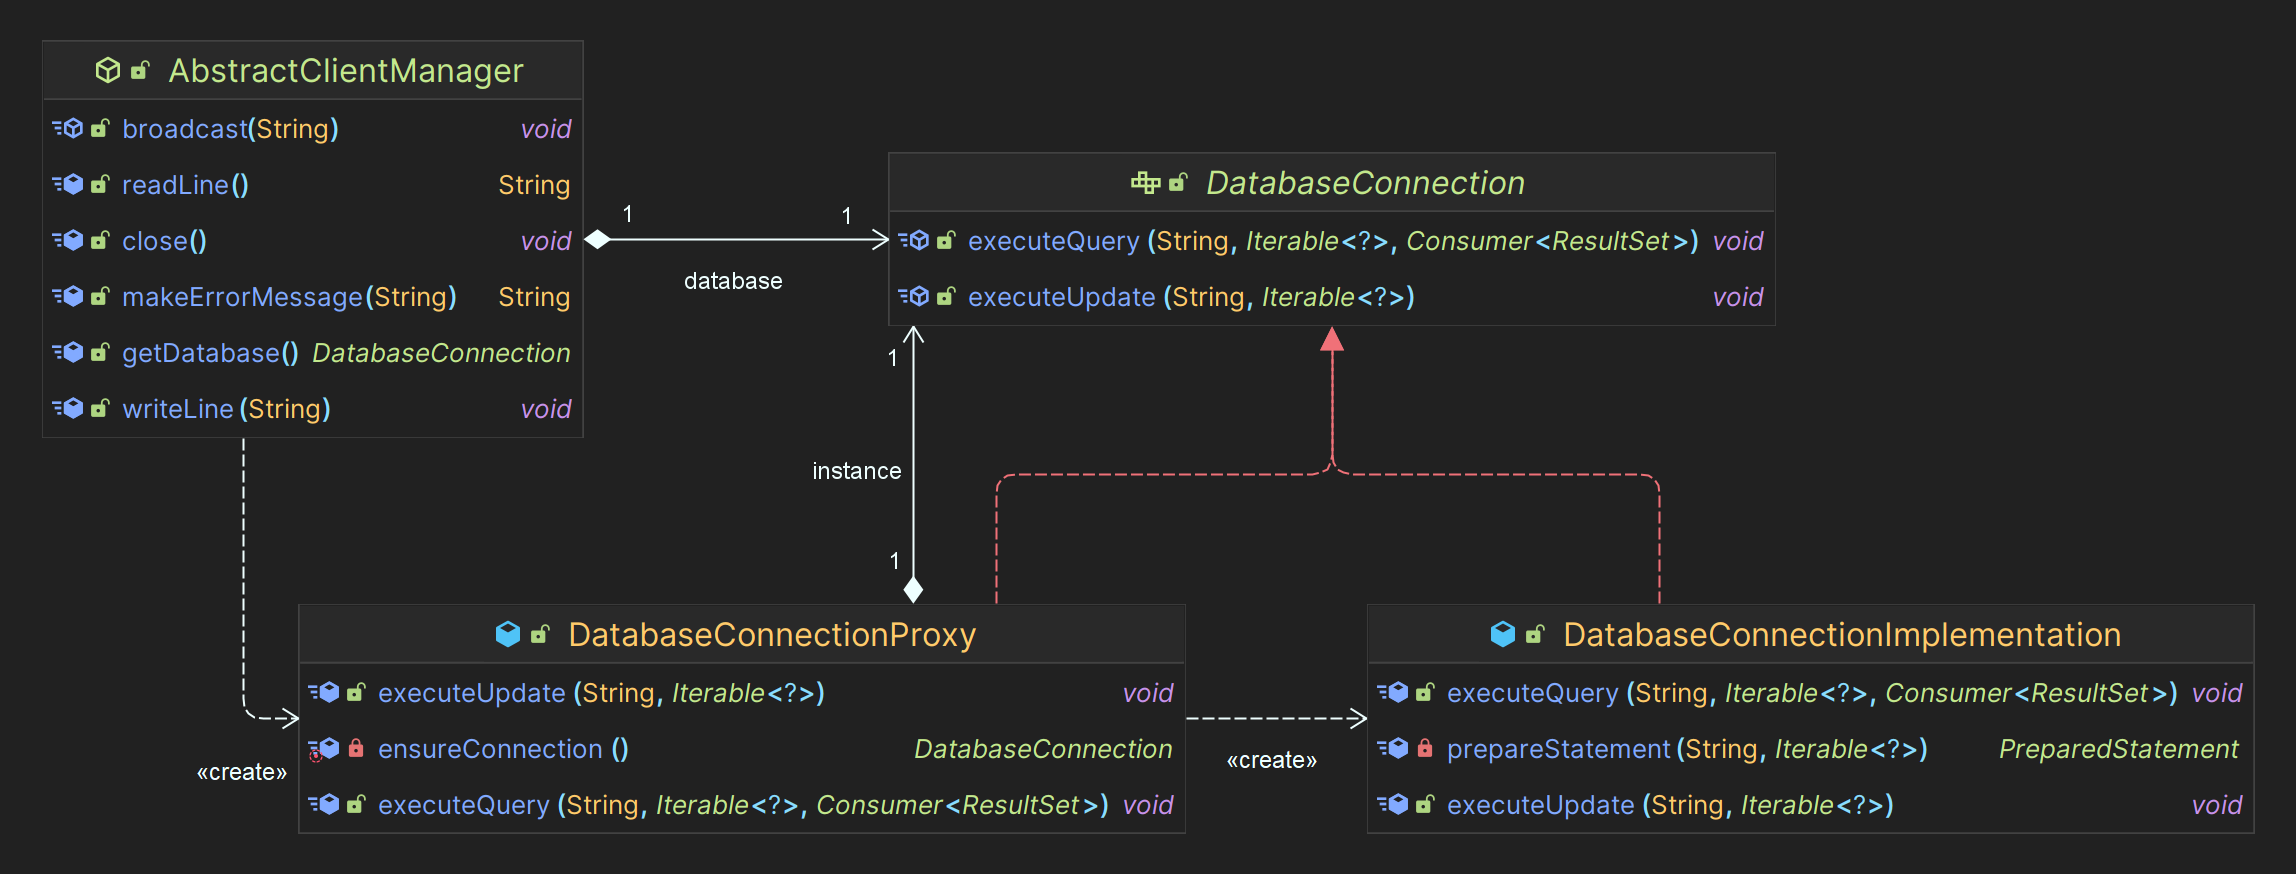
\includegraphics[width=\textwidth,height=\textheight,keepaspectratio]{ProxyUMLdetailed.png}
    \caption{Struttura Proxy pattern implementato nel SW con metodi}
\end{figure}

\subsection{Strategy}

\noindent Questo pattern behavioural definisce una famiglia di algoritmi, incapsulandoli e rendendoli intercambiabili. Si usa quando si ha necessità di modificare dinamicamente gli algoritmi utilizzati dall’applicazione.\\
\textit{N.B.:} L’algoritmo cambia indipendentemente dai client che lo usano

\subsubsection{Utilizzo pratico}
\noindent Nel nostro caso, questo pattern è stato utilizzato per implementare facilmente la gestione dei  comportamenti dei vari server, questi forniscono funzionalità diverse e gestiscono messaggi diversi ma, alla base delle loro funzionalità c’è sempre lo stesso principio: lo scambio di messaggi.

\begin{figure}[htbp]
    \centering
    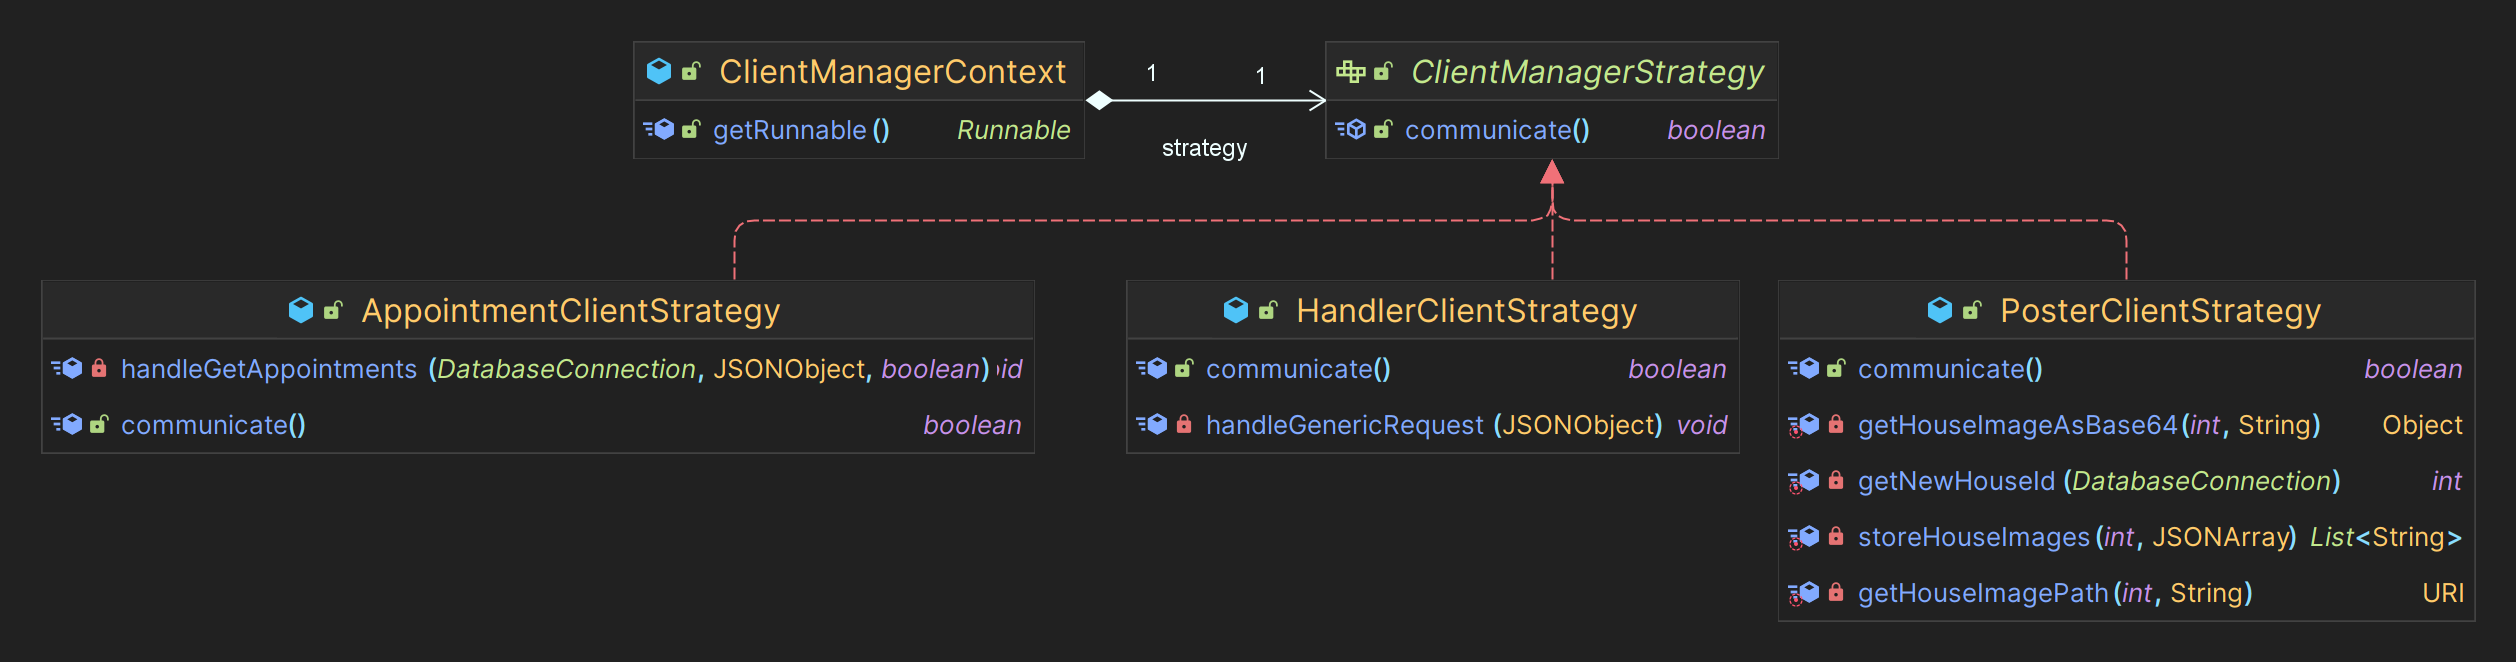
\includegraphics[width=\textwidth,height=\textheight,keepaspectratio]{StrategyUMLdetailed.png}
    \caption{Struttura Strategy pattern implementato nel SW con metodi}
\end{figure}
\chapter{Architettura}
\noindent Il sistema impiega un’architettura di tipo \textbf{ibrido}, utilizzando sia caratteristiche del modello \textbf{client/server} chee quelle del modello \textbf{peer-to-peer}.\\
In dettaglio, la struttura prevede l’utilizzo di tre server:
\begin{itemize}
    \item \textbf{Handler Server:} coordina la comunicazione tra il client e gli altri due server;
    \item \textbf{Poster Server:} svolge funzioni di gestione degli \textit{annunci};
    \item \textbf{Appointment Server:} svolge funzioni di gestione degli \textit{appuntamenti}.
\end{itemize}
La connessione è effettuata tramite \textbf{Socket}, con protocollo \textbf{TCP/IP}, risultando quindi \textit{connection-oriented} e \textit{reliable}.
Possiamo dividere l’architettura in quattro processi:
\begin{itemize}
    \item \textbf{Main Client:} agisce puramente da client e si interfaccia esclusivamente con il processo “Handler Server”, sia per l’autenticazione che per la comunicazione con gli altri due processi;
    \item \textbf{Handler Server:} agisce sia da server, verso il processo “Handler Server” che da client, verso di processi “Poster Server” e “Appointment Server”.\\
    Si occupa principalmente di smistare i messaggi in arrivo dal processo “Main Client” e di gestire l’autenticazione con lo stesso;
    \item \textbf{Poster Server:} agisce puramente da server, verso il processo “Handler Server”.\\
    Si occupa di gestire i comandi riguardanti gli immobili, ossia inserimento, cancellazione e selezione.;
    \item \textbf{Appointment Server:} agisce puramente da server, verso il processo “Handler Server”.\\
    Si occupa di gestire i comandi riguardanti gli appuntamenti, ossia inserimento, cancellazione e selezione..
\end{itemize}

\chapter{Comunicazione}
\noindent La comunicazione tra le varie entità del sistema è eseguita tramite \textbf{primitive bloccanti} per \texttt{read} e per \texttt{write}, nel caso di Java, \texttt{writeLine} e \texttt{readLine}. Lo scambio di messaggi avviene in \textbf{locale} basandosi sul protocollo \textbf{TCP/IP} tramite l'utilizzo di socket \textbf{bidirezionali}; pertanto, sarà sufficiente utilizzare una singola socket per ogni client connesso.\\
\\
\noindent Quando viene \textbf{inviato} un messaggio, questo viene posto in un \textbf{buffer interno}: qualora il buffer dovesse essere \textit{pieno}, il thread è bloccato finché non si \textit{svuota}.\\
Al fine di garantire questo comportamente, viene utilizzato il tipo \texttt{PrintWriter}, configurato con \texttt{autoFlush}.\\
\textit{N.B.:} il messaggio viene processato prima di essere inviato, aggiungendo simboli di escape.\\
\\
Quando viene \textbf{ricevuto} un messaggio, il thread è bloccato in attesa di un messaggio da leggere, una volta che il messaggio è presente sullo stream di input, viene processato rimuovendo i simboli di escape e inserito in una struttura dati \texttt{JSON}.\\
\\
\noindent Per design, è assunto che il contenuto e la struttra dei messaggi in JSON siano validi e NON è per tanto necessario eseguire operazioni di controllo.\\
Verranno però validati i parametri inviati dal client.

\section{$\text{Main Client} \Leftrightarrow \text{Handler Server}$}
\noindent Il client principale si interfaccia con l’Handler Server per autenticarsi, e per la comunicazione con gli altri server.\\
L’istante in cui un client si connette all’Handler Server, questo genera automaticamente altre due connessioni ai server ausiliari; a questo punto i tre server si mettono in attesa di messaggi.\\
La comunicazione diretta per l’autenticazione viene effettuata specificando nel campo \texttt{type} della richiesta “generic”.
\section{Autenticazione - \texttt{handleSignInRequest}}
\noindent All’avvio del client, viene mostrata una finestra di login dove l’utente potrà inserire il suo username e la sua password, una volta confermati i dati, l’applicazione costruirà una richiesta \texttt{JSON} con i parametri necessari al login e verrà inviata immediatamente al server.\\Il client si mette poi in attesa di una risposta dal server, se questa contiene i privilegi di accesso allora il login avrà avuto successo, altrimenti la risposta conterrà un errore con una breve spiegazione del problema.

\section{Registrazione - \texttt{handleSignUpRequest}}
\noindent Dalla schermata di login, viene mostrato un bottone che permette di registrarsi, la registrazione richiede all’utente di inserire:
\begin{itemize}
    \item Username;
    \item Password;
    \item Nome;
    \item Cognome.
\end{itemize}
Una volta confermati i dati, l’applicazione costruisce una richiesta \texttt{JSON} con i parametri necessari per la registrazione e la invia immediatamente al server.\\
A questo punto, il client si mette in attesa di una risposta dal server. Se la risposta contiene un \texttt{JSON} vuoto, l’utente viene registrato nel sistema. In caso contrario, la risposta conterrà un errore con una breve spiegazione del problema (es. l’username scelto è già in uso).

\section{$\text{Main Client} \Leftrightarrow \text{Handler Server}$}
\noindent L’Handler Server gestisce la comunicazione con il Poster Server internamente e in maniera trasparente all’utente. I messaggi aventi il campo type impostato a “poster” vengono inoltrati automaticamente a questo server.\\
Le richieste supportate dal Poster Server sono:
\begin{itemize}
    \item \texttt{getHouses};
    \item \texttt{insertHouse};
    \item \texttt{deleteHouse}.
\end{itemize}

\section{Richiesta di Immobili – \texttt{getHouses}}
\noindent Questa richiesta viene effettuata immediatamente quando \texttt{MainViewController}, ossia la pagina principale dell’applicazione, viene mostrata; oppure quando si cambia pagina verso \texttt{MainViewController}.\\
Questa richiesta non ha bisogno di parametri e si limita a restituire l’intera collezione di immobili disponibili nel database come un array \texttt{JSON}.\\
Non essendo previsti errori per questa richiesta, possiamo assumere che andrà sempre a buon fine.

\section{Inserimento di Immobili – \texttt{insertHouse}}
\noindent La richiesta di inserimento di un immobile gestisce sia l’inserimento che la modifica degli stessi. Viene originata da \texttt{AddHouseController}, ossia la pagina di inserimento e modifica immobili.\\
\\
La richiesta dovrà contenere tutti i parametri necessari per l’inserimento di un immobile, con eventuali parametri opzionali come le immagini da inserire e l’id per l’immobile.\\
Quest'ultimo risulta opzionale in quanto, quando la richiesta contiene l’id, viene interpretata come una modifica.\\
\textit{N.B.:} Qualora un immobile non abbia una o più immagini, ne verrà utilizzata una placeholder.\\
Le immagini sono trasmesse dal server e al client in formato \textbf{base64}.\\
Non essendo previsti errori per questa richiesta, possiamo assumere che andrà sempre a buon fine.

\section{Cancellazione di Immobili – \texttt{deleteHouse}}
\noindent La richiesta di cancellazione di un immobile è originata da \texttt{AddHouseController} e necessita solo di un parametro, l’id dell’immobile da eliminare.\\
Poiché l’amministratore non specifica mai manualmente l’id (in quanto automaticamente determinato da \texttt{AddHouseController}), si può assumere che questo sia sempre valido, pertanto, tale funzione non restituisce nessun errore.

\section{$\text{Handler Server} \Leftrightarrow \text{Appointment Server}$}
\noindent L’Handler Server gestisce la comunicazione con l’Appointment Server internamente e in maniera \textit{trasparente} all’utente. I messaggi che hanno il campo \texttt{type} impostato ad “appointment” vengono inoltrati automaticamente a questo server.\\

\section{Richiesta Appuntamenti – \texttt{getAppointmentsForUser / Agent}}
\noindent Questa richiesta acquisisce gli appuntamenti per l’utente specificato, il quale può essere sia un cliente che un agente immobiliare. La richiesta è originata da \texttt{MainViewController} automaticamente.\\
In base al tipo di utente attualmente loggato, viene richiamata la funzione\\ \texttt{getAppointmentsForUser} o \texttt{getAppointmentsForAgent}.\\
Sarà ritornata una lista di appuntamenti presi dall’utente oppure la lista di appuntamenti a cui partecipa l’agente sottoforma di array \texttt{JSON}. Si può inoltre assumere che non saranno ritornati errori.

\section{Richiesta Appuntamenti – insertAgentAvailability}
\noindent Questa richiesta è originata da \texttt{InsertAvailabilityController} ed inserisce un range di disponibilità in base ai parametri \texttt{start\_date} e \texttt{end\_date}.\\
Le date saranno inserite una ad una nel database e, nel caso una data sia già presente, sarà semplicemente saltata.\\
Poiché il controllo \texttt{end\_date > start\_date} è effettuato dal client, si può assumere che non saranno ritornati errori.

\section{Richiesta Appuntamenti – \texttt{bookAppointment}}
\noindent Questa richiesta è originata da \texttt{HouseDetailsController}, in questo caso, l’utente loggato, ossia il cliente, vuole riservare un appuntamento per un immobile scegliendo il primo agente disponibile.\\
La funzione ritorna due errori che devono essere obbligatoriamente gestiti dal client; in entrambi i casi l’appuntamento NON è prenotato e la disponibilità dell’agente rimane invariata.
Gli errori sono:
\begin{itemize}
    \item \textbf{\texttt{notAvailable}:} Se l’utente sceglie una data dove nessun agente ha dato disponibilità;
    \item \textbf{\texttt{alreadyBooked}:} Se l’utente sceglie una data per cui ha già preso un appuntamento. 
\end{itemize}

\section{Richiesta Appuntamenti – removeAppointment}
\noindent Questa richiesta è originata da \texttt{MainViewController} quando l’utente, ossia il cliente, vuole cancellare un appuntamento. La funzione richiede un solo parametro: l’id dell’appuntamento da rimuovere.\\
Poiché l’utente può solo cancellare un appuntamento che appare nella lista di appuntamenti, si può assumere che l’id sarà sempre valido, pertanto la richiesta non ritorna errori.
\def\baselinestretch{1}
\chapter{Database} \label{db}
\def\baselinestretch{1.66}

\noindent Come sopracitato, è stato utilizzato SQLite in quanto la natura embedded permette di incorporarlo direttamente nell'applicazione, rendendo la gestione dei dati più agevole e contribuendo a ridurre la complessità della configurazione del sistema. Questo è particolarmente vantaggioso per un'applicazione di medie dimensioni come la nostra.\\
\noindent Segue il diagramma relazionale del database impiegato come fondamento per la memorizzazione a lungo termine dei dati del software.

\begin{figure}[h]
\centering
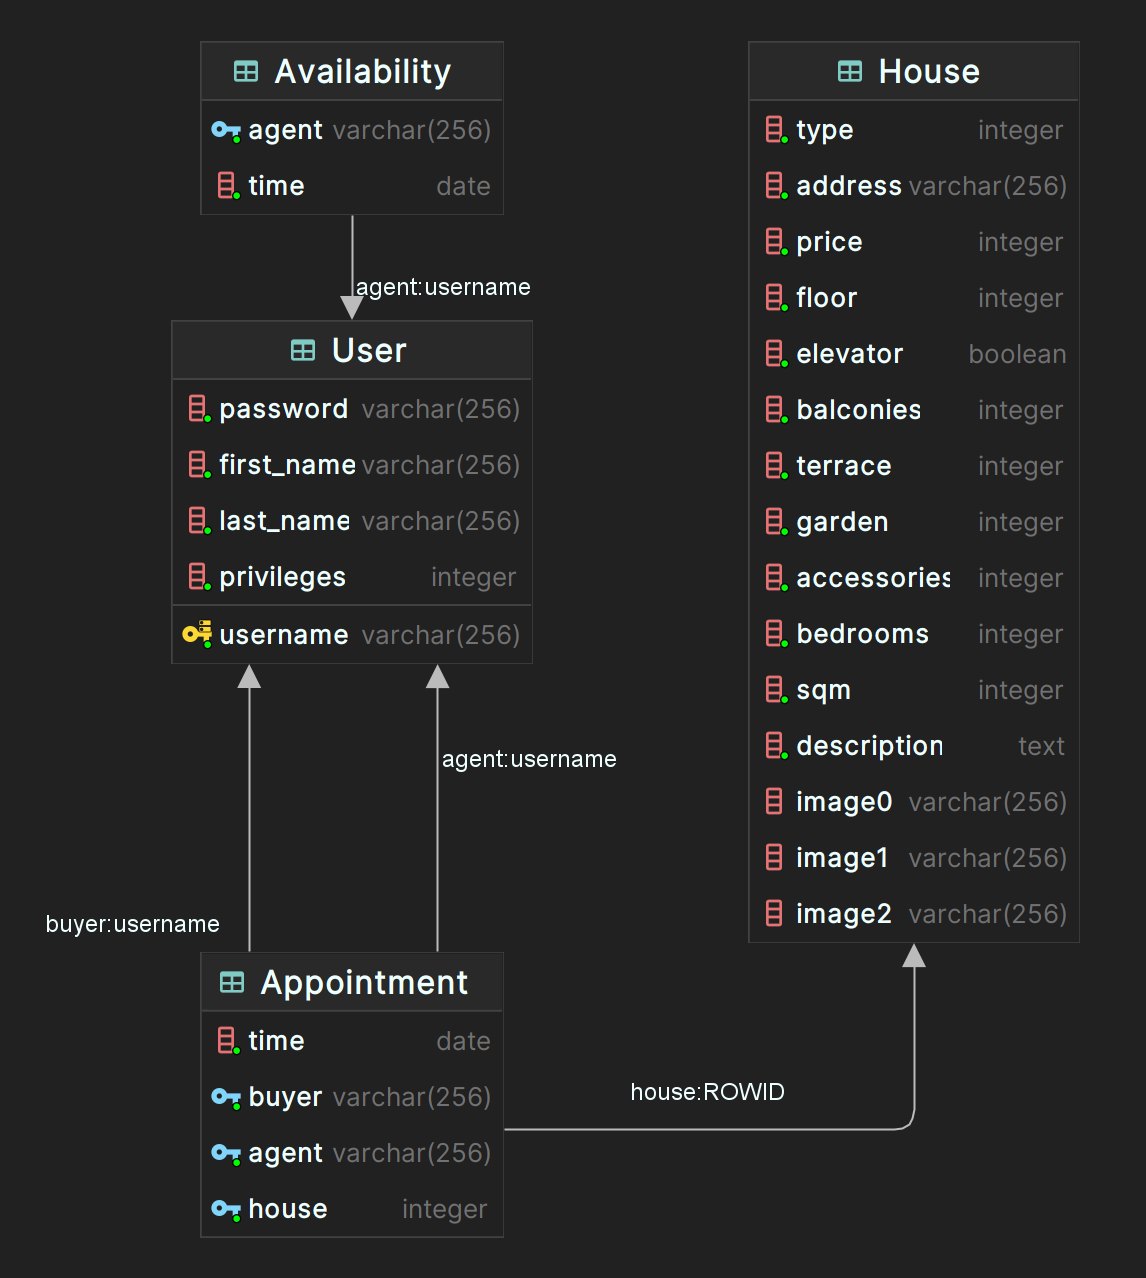
\includegraphics[scale=0.3]{properteaseDB.png}
\caption{Diagramma relazionale del database}
\end{figure}
\chapter{Guida all'utente}
\section{Avvio dell'applicazine}
\noindent Per poter utilizzare l'applicativo in maniera corretta bisogna
\begin{enumerate}
    \item Avviare il processo server "\texttt{StartServer}";
    \item Avviare il processo client "\texttt{StartApplication}".
\end{enumerate}

\section{Accesso}
\noindent Per assegnare il ruolo di "Amministratore" a un utente, è necessario effettuare l'inserimento direttamente nel database per garantire un adeguato controllo dei privilegi e una buona gestione degli accessi.\\
\\
Per utilizzare l'applicazione, sia il cliente che l'amministratore (agente immobiliare) devono effettuare l'accesso. Tale procedura richiede l'inserimento di un nome utente e di una password.\\
Al momento del tentativo di accesso, il sistema, tramite il \texttt{Main Handler} interroga il database per verificare se l'utente è registrato e se le credenziali inserite sono corrette.\\

\begin{figure}[h]
\begin{tabular}{ll}
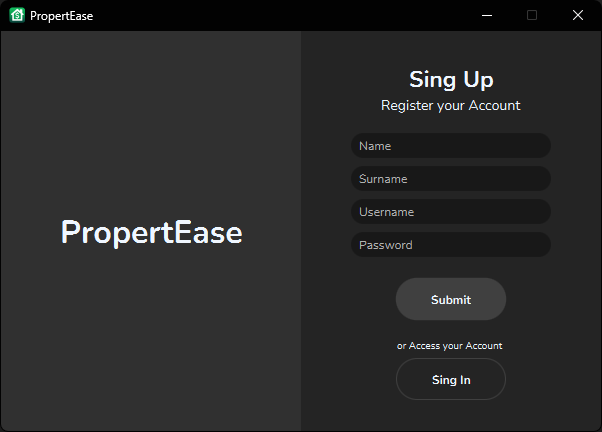
\includegraphics[scale=0.35]{signup.png}
&
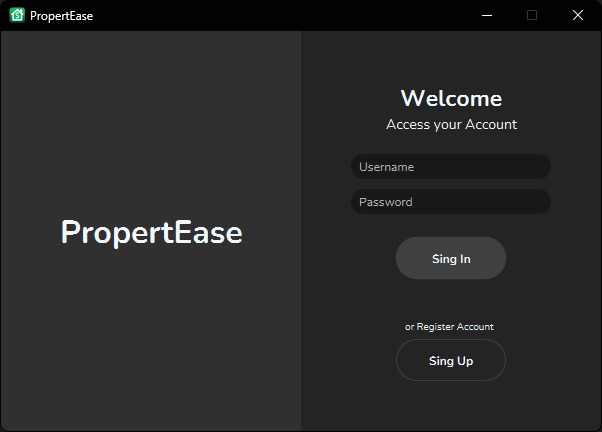
\includegraphics[scale=0.35]{login.png}
\end{tabular}
\caption{(sx): registrazione (dx): accesso}
\label{Fig:Race}
\end{figure}

\noindent Nel caso in cui un utente non risulti registrato, è possibile effettuare la registrazione tramite la sezione dedicata denominata "Sign Up". In questa sezione, vengono richiesti il nome, il cognome, il nome utente e la password.\\
\textit{N.B.:} Sono implementati controlli sull'unicità del nome utente. Se i dati inseriti sono corretti, le credenziali vengono memorizzate nel database.
\section{Utilizzo applicazione}
\subsection{Utente}
\noindent L'interfaccia utente post-login è molto intuitiva, con le card cliccabili per ogni immobile ed un tab sulla sinistra con i suoi appuntamenti.\\
\\
Cliccando su una della card, si è reindirizzati alla pagina in cui sono mostrati i dettagli degli immobili e dove  è possibile prenotare un appuntamento.\\
\\
La navbar in alto permette la navigazione delle pagine.

\begin{figure}[htbp]
    \centering
    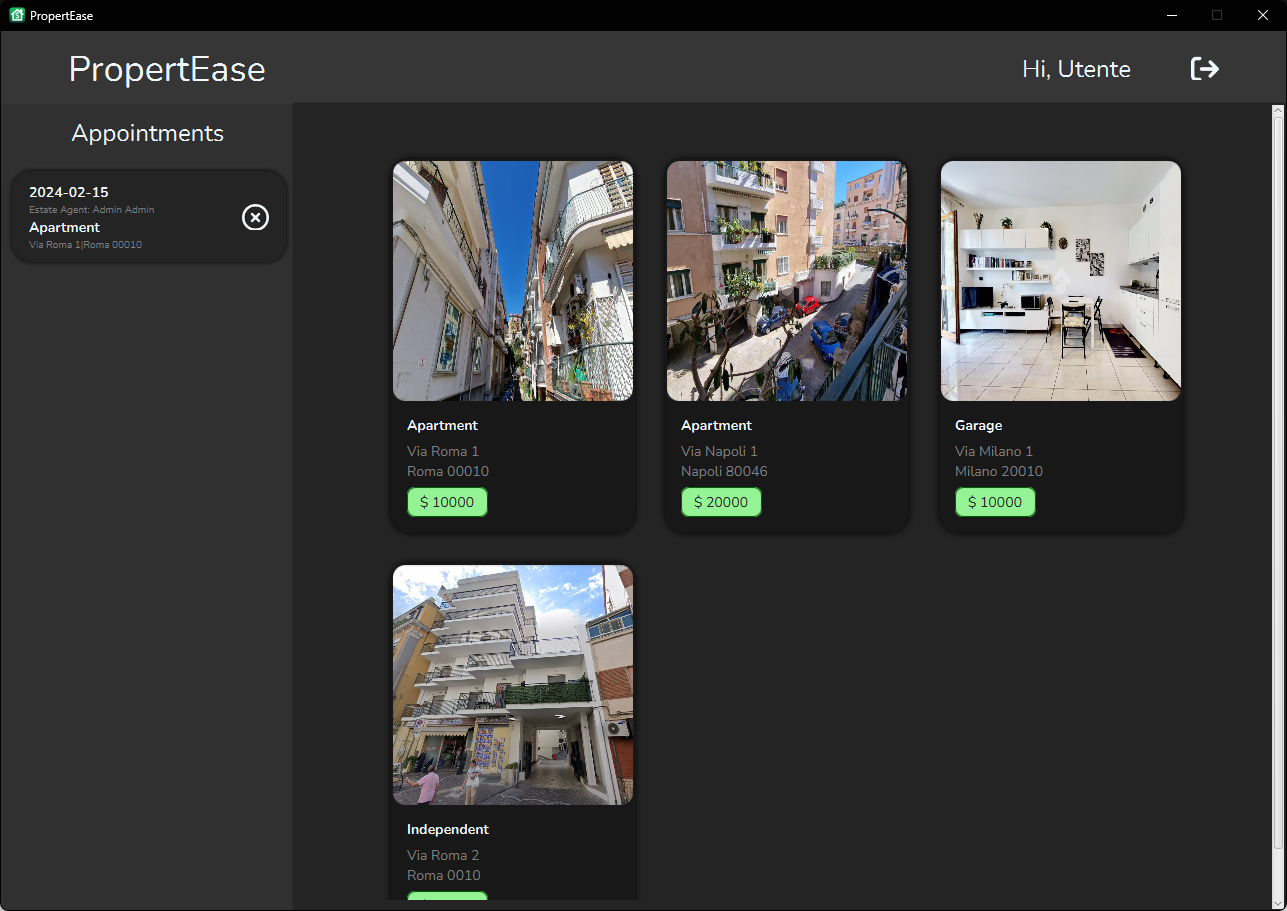
\includegraphics[width=\textwidth,height=\textheight,keepaspectratio]{mainDashboard.png}
    \caption{Schermata principale dell'applicazione}
\end{figure}
\begin{figure}[htbp]
    \centering
    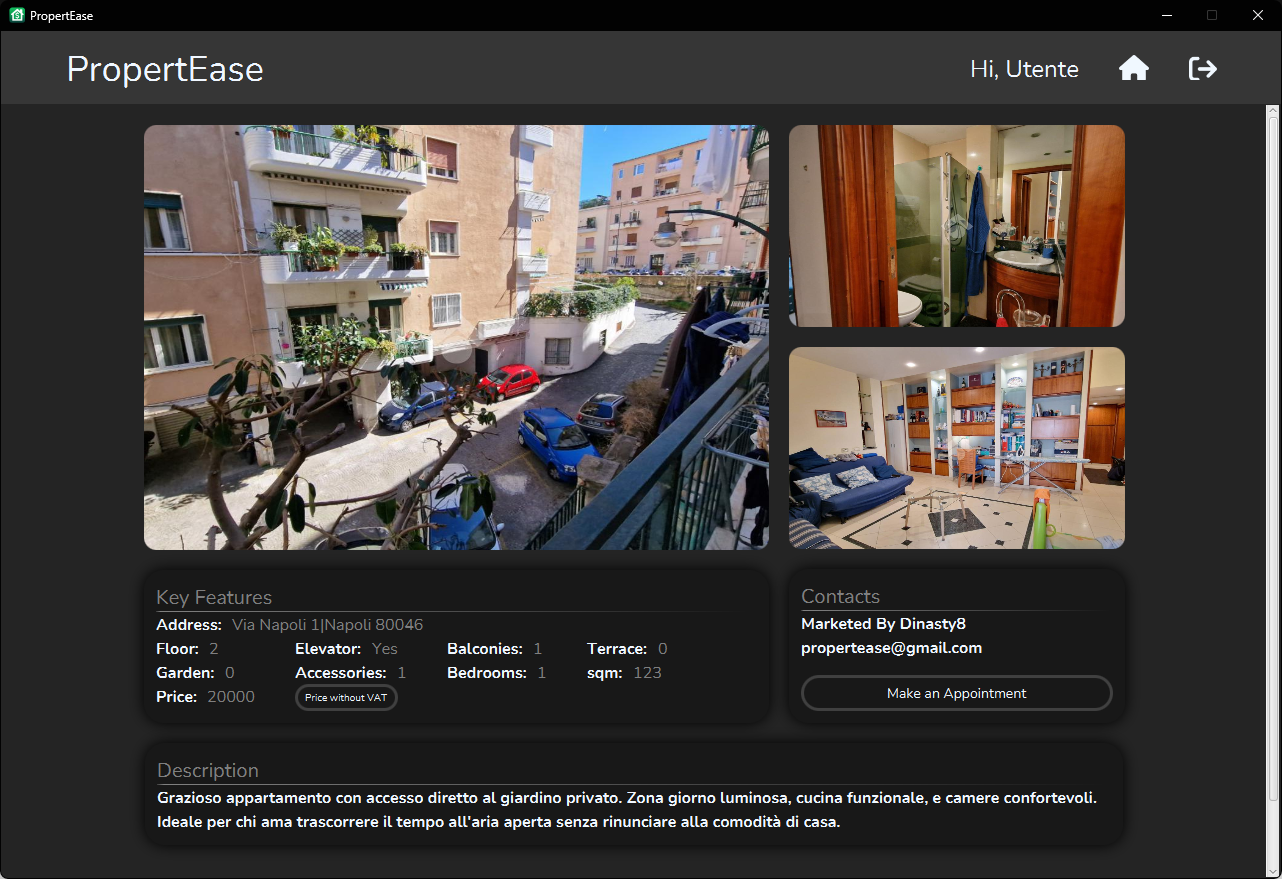
\includegraphics[width=\textwidth,height=\textheight,keepaspectratio]{houseView.png}
    \caption{Schermata dei dettagli di un immobile}
\end{figure}

\subsection{Amministratore}
\noindent Oltre a quanto sopracitato per l'utente, l'amministratore avrà le varie funzioni sempre in pulsanti locati in alto a destra della GUI.\\
Tramite questi bottoni, egli potrà inserire, rimuovere e aggiornare gli immobili del database.\\

\subsection{Errori}
\noindent per ogni operazione di modifica, inserimento ed eliminazione su database, è stato inserito, dal punto di vista di interfaccia, un pop-up di conferma o metodi di ripristino dei dati.

\begin{figure}[h]
\begin{tabular}{ll}
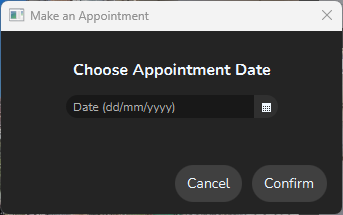
\includegraphics[scale=0.65]{takeAppointment.png}
&
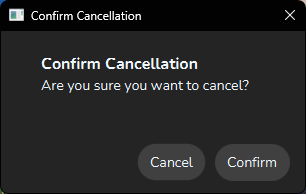
\includegraphics[scale=1]{confirmCancellation.png}
\end{tabular}
\caption{conferma di presa (sx) e cancellazione (dx) di un appuntamento}
\label{Fig:Race}
\end{figure}

\newpage
\pagestyle{plain}

\end{document}
